We consider a gas of $N_p$ bosons in spherical and elliptical harmonic oscillator potentials. The interaction between bosons is modeled by the hard-core model as in \cite{vmcarticle}. %We set $\hbar = m = 1$. 
The Hamiltonian of the system is 
\begin{equation}
H = \sum_{i=1}^{N_p}\left[ -\frac{1}{2}\frac{\hbar^2}{m}\nabla_i^2 + V_{ext}(\textbf{r}_i) \right]+ \sum_{i \neq k} V_{int}(r_{ik}),
\label{eq_hamilton}
\end{equation}
where $V_{ext}(\textbf{r})$ is the harmonic oscillator potential given by
\begin{equation*}
V_{ext}(\textbf{r})=\begin{cases}
\frac{1}{2}m\omega_{ho}^2r^2 &\text{Spherical}\\
\frac{1}{2}m\left[ \omega_{ho}^2 \left(x^2 + y^2 \right) + \omega_z^2 z^2\right] &\text{Elliptical}
\end{cases}
\end{equation*}
and $V_{int}(r_{ik})$ is the hard-core interaction potential 
\begin{equation*}
V_{int}(r_{ik}) = \begin{cases}
 0, & r_{ik} > a \\
 \infty, & r_{ik} < a.
\end{cases}
\end{equation*}
The quantity $r_{ik} = |\textbf{r}_i-\textbf{r}_k|$ represents the distance between particle $i$ and $k$, while $a$ is the size of the interaction between particles. 

\paragraph{No interaction - spherical trap} When we set the interaction to be zero ($V_{int}=0$), we are left with a harmonic oscillator potential, where we consider a spherical shape for simplicity. In this case the solutions are known analytically. In general the energy is given by $E_n=\hbar\omega_{ho}(n+\frac{1}{2})$. The ground state is 
\begin{equation*}
E(N_p,\text{D}) = \frac{1}{2}\text{D} N_p\ \hbar\omega_{ho}.
\label{analitica}
\end{equation*}
where D is the dimension of the system and $N_p$ is the number of particles. This case is useful to benchmark our code at the beginning.

\subparagraph{No interaction - elliptical trap}
The interaction is still null ($V_{int}=0$), the trap now is considered to be elliptical.\\
Let us introduce lengths in unit of $a_{ho}=\sqrt{\hbar/(m\omega_{ho)}}$, $r\rightarrow r/a_{ho}$ and energy in units of $\hbar\omega_{ho}$. The Hamiltonian can be rearranged as 
\begin{equation*}
\begin{split}
H&=\sum_{k=1}^{N_p}\bigg(-\frac{\hbar^2}{2m}\nabla^2_{k}+\frac{1}{2}m[\omega^{2}_{ho}(x^2_k+y^2_k)+\omega^{2}_{z}z_k^2]\bigg)\\
&=\sum_{k=1}^{N_p}\frac{\hbar \omega_{ho}}{2}\bigg(-\frac{\hbar}{m\omega_{ho}}\nabla^2_{k}+\frac{\omega_{ho}m}{\hbar}\bigg[x^2_k+y^2_k+\frac{\omega^{2}_{z}}{\omega^{2}_{ho}}z^2_k\bigg]\bigg)\\
&=\sum_{k=1}^{N_p}\frac{\hbar \omega_{ho}}{2}\bigg(-a_{ho}\nabla^2_{k}+a_{ho}{\hbar}\bigg[x^2_k+y^2_k+\frac{\omega^{2}_{z}}{\omega^{2}_{ho}}z^2_k\bigg]\bigg).
\end{split}.
\end{equation*}
We set $\lambda=\omega_z/\omega_{ho}$, we get
\begin{equation}
\label{ham}
H=\sum_{k=1}^{N_p}\frac{1}{2}\bigg(-\nabla^2_{k}+V_{ext}(\mathbf{r}_k)\bigg)
\end{equation}
where $V_{ext}=x^2_k+y^2_k+\lambda^2 z^2_k$. As in \cite{DalfString}, we set $\lambda=\sqrt{8}$. In \cite{vmcarticle}, the energy of non-interacting bosons in this trap is shown to be

\begin{equation*}
	\frac{E}{N}\rightarrow E_{ho}=\hbar\omega_{ho}\bigg(1+\frac{\lambda}{2}\bigg)=2.414\ \hbar\omega_{ho}.
\end{equation*}

We will use this result to benchmark again our code.

\subparagraph{Interaction - elliptical trap}
At this point, we turn on the interaction $V_{int}\neq 0$ and we consider an elliptical trap. The Hamiltonian is

\begin{equation}
\label{ham2}
H=\sum_{k=1}^{N_p}\frac{1}{2}\bigg(-\nabla^2_{k}+V_{ext}(\mathbf{r}_k)\bigg)+\sum_{k<i}^{N_p} V_{int}(\mathbf{r}_k,\mathbf{r}_i).
\end{equation}
where $V_{ext}=x^2_k+y^2_k+\lambda^2 z^2_k$ and $\lambda=\sqrt{8}$ as above.
%\noindent During the whole project, we will use natural units $\hbar=m=\omega_{ho}=1$.

\section{Methods}
To compute the ground state energy of bosons, we use the variational method from quantum mechanics which gives an upper bound for the ground state energy $E_{gs}$ given a trial wave-function $\Psi_T$: 
\begin{equation}
\label{var_princ}
E_{gs}\leq \frac{\braket{\Psi_T|H|\Psi_T}}{\braket{\Psi_T|\Psi_T}}\boldsymbol=\frac{\int \Psi_T^{*}(\textbf{X},\boldsymbol{\theta})H\Psi_T(\textbf{X},\mathbf{\theta})d\textbf{X}}{\int \Psi_T^{*}(\textbf{X},\boldsymbol{\theta})\Psi_T(\textbf{X},\boldsymbol{\theta})d\textbf{X}}.
\end{equation}
In eq. (\ref{var_princ}), $\mathbf{X}$ represents the particles' positions and $\boldsymbol{\theta}$ represent the variational parameters. With Machine Learning, the variational parameters are the biases of the NN. Hence $\boldsymbol{\theta} = a_1, \dots, a_\text{N},  b_1, \dots, b_\text{M}, w_{11}, \dots, w_{\text{NM}}$. The quantities N and M are respectively the number of visible and the number of hidden nodes. \\
The integral in eq. (\ref{var_princ}) is impossible to evaluate with methods such as Gaussian quadrature in a reasonable amount of time. In such a situation, Monte Carlo methods are needed.

Let us consider a trial wave-function and define the probability density function (PDF) 
\begin{equation}
\label{PDF}
P(\mathbf{X},\boldsymbol{\theta})=\frac{|\Psi_T|^2}{\int d\textbf{X}|\Psi_T|^2}
\end{equation}
and define the local energy as
\begin{equation}
\label{local_energy}
E_L=\frac{1}{\Psi_T}H\Psi_T.
\end{equation}
By using eq. (\ref{PDF}) and eq. (\ref{local_energy}), we have
\begin{equation*}
E_{gs}\leq  \frac{\int d\mathbf{X} \Psi^{*}_{T}H\Psi_T}{\int d\mathbf{X}|\Psi_T|^2}=\int d\mathbf{X}\  P(\mathbf{X},\boldsymbol{\theta})E_L(\mathbf{X},\boldsymbol{\theta})\simeq \frac{1}{N_{MC}}\sum_{i=1}^{N}P(\mathbf{X}_i,\boldsymbol{\theta})E_L(\mathbf{X}_i,\boldsymbol{\theta})
\end{equation*}
where $N_{MC}$ is the number of Monte Carlo steps.

%With the basic VMC method, our variational parameter is represented by a value which we call $\alpha$. Therefore to find the minimum energy we can use MC methods to compute the mean local energy for different alphas and then see which alphas return the minimum energy. An automated version of this is to use numeric methods that finds function minimums based on the calculations from the MC cycles. For instance conjugate gradient and gradient descent are good iterative methods. We will implement the gradient descent method: the outline is to do some MC cycles to calculate quantities needed for the numeric minimum finder per iteration, eventually the numeric method will find a minimum and return an optimal $\alpha$. Then we can do MC sampling with many more steps on the system with the optimal parameters. This is a proper variational Monte Carlo \cite{morten_book} (VMC) method. 

We will use MC methods to calculate the local energy for a set of Gaussian distributed $\boldsymbol{\theta}$, then we will apply the Stochastic Gradient Method (SGD) (more in section \ref{sec_SGD}) to find a new $\boldsymbol{\theta}$ that will give a lower energy. This is an iterative method to find a function minimum. The final result should be a good estimate for the ground state. Since the SGD method has to be applied many times, the number of MC cycles for each SGD iteration should not be very large (to save time). Rather once the SGD cycles have finished we do a run of the final set of parameters with a large number of MC cycles to give a final answer.

However this method will not always be applicable. If the RBM is not able to converge to a precise energy but notably fluctuates, then it is not meaningful to use a final set of variational parameters for a final MC run. Instead the SGD local energy is used. We average the SGD data after equilibration. This will produce a mean local energy that can be used as a final result.

\subsection{Sampling methods}
We use MC methods to measure system quantities such as energy by generating samples that reproduce more and more precisely the desired distribution. The basic recipe is to choose one particle randomly, and propose in a certain way a step for that particle. Then according to a certain rule either accept or decline the move. We will use two methods to propose and accept/reject moves: Brute-Force Metropolis (BFM) and Importance Sampling Metropolis-Hastings (ISMH) \cite{morten_book}. 

\subsubsection{Brute-Force Metropolis algorithm}
The standard Metropolis algorithm (also referred to as Brute-Force Metropolis in this text) follows the basic recipe (referred to as a "brute-force" sampling rule) for choosing new positions given by
\begin{equation*}
x_{k+1} = x_k + Lr,
\end{equation*}
where $L$ is a step length and $r$ is a uniformly distributed random variable $\in [0,1]$. We accept moves that are deemed likely by the ratio of the absolute square wave-functions before and after the move. We choose a new random number r, and if
\begin{equation}
r \leq \frac{|\Psi_T(\textbf{r}_{k+1})|^2}{|\Psi_T(\textbf{r}_{k})|^2},
\label{eq_accept_move}
\end{equation}
then we accept the move. If it is not verified, we decline it. 

\subsubsection{Importance Sampling Metropolis-Hastings algorithm}
The issue with BFM is that the algorithm proposes a lot of moves that get rejected. The independence of the sampling rule with respect to the trial wave-function is responsible for this behaviour. These rejected moves cause a lot are wasted computation time and as such, it becomes desirable to use an algorithm that proposes moves that are more likely to be accepted. In order to obtain this, we will use the Importance Sampling way of generating samples.

The basic idea behind Importance Sampling is to propose moves corresponding to an isotropic diffusion
process with a drift. Such a process obeys Fokker-Planck equation 
\begin{equation*}
\frac{\partial P}{\partial t} = D\frac{\partial}{\partial x}\left(\frac{\partial}{\partial x}-F\right)P,
\end{equation*}
where $P$ is the probability density function of the system, $D$ is the diffusion coefficient and $F$ is the drift force. This equation governs the time evolution of the probability density function for a diffusing system under random forces. In the bosonic system the probability density function is the wave-function itself and we call $F$ the quantum force. The diffusion coefficient assumes the value $1/2$ ($D = 1/2$) due to the half factor in the kinetic energy. 

The solution of the Fokker-Planck equation is 
\begin{equation*}
F = \frac{2\nabla \Psi_T}{\Psi_T}.
\end{equation*}
and the new move is given by the following sampling rule
\begin{equation*}
x_{k+1} = x_k + DF\Delta t + r\sqrt{\Delta t},
\end{equation*}
where $\Delta t$ is some time step parameter that can be tuned. 

Now that we have changed the sampling rule we need to alter the method of accepting/rejecting such moves. We move then to the Metropolis-Hastings algorithm. The probability of diffusion can be solved from the Fokker-Planck equation through a Green function
\begin{equation*}
G(x_{k+1},x_k,\Delta t) = \frac{1}{(2\pi\Delta t)^{3N/2}}\exp\left[ -\frac{\left(x_{k+1} - x_{k} - \Delta tF(x_k)\right)^2}{2\Delta t}  \right].
\end{equation*}
The new moves are now accepted following the rule 
\begin{equation}
r \leq \frac{G(x_k, x_{k+1}, \Delta t)|\Psi_T(x_{k+1})|^2}{G(x_{k+1}, x_{k}, \Delta t)|\Psi_T(x_{k})|^2},
\label{eq_imp_sam}
\end{equation}
where $r$ is a Gaussian distributed random number. 

\subsection{Iterative methods to find optimal variational parameters}
In order to obtain the minimum energy, we need to adjust the variational parameters $\boldsymbol{\theta}$.% for the ML case.
Therefore we introduce the Stochastic Gradient Descent (SGD) method.

%\subsubsection{Gradient descent}
%Sometimes referred to as steepest descent, the gradient descent method is an iterative method used to find local minima of functions. The basic idea is to choose an initial $\textbf{x}$ and find a new $\textbf{x}$ following
%\begin{equation*}
%\textbf{x}_{k+1} = \textbf{x}_{k} - \lambda_k \nabla f(\textbf{x}_k),
%\end{equation*}
%where $\lambda_n$ is some factor, preferably small. If the derivative is negative, then $x$ will increase. If the derivative is positive, $x$ will decrease. At the minimum the derivative will be zero and thus the method will converge. There are many gradient descent methods which differ by choice of $\lambda_n$. The ideal method is to have some algorithm such that $\lambda$ approaches zero when the function approaches the minimum. This project will use constant $\lambda$. The simple algorithm can be implemented as
%\begin{lstlisting}
%while (iter < maxIterations && energyDerivative < tolerance){	
%x -= lambda*gradF(x)
%}	
%\end{lstlisting} 
%An issue with the gradient descent method is that it can only find local minimum without knowing whether it is the global one or not. This can be bypassed by running the algorithm multiple times with different initial guesses. If they converge to the same minimum, it is a good indication that the function only has one local(global) minimum. 

\subsubsection{Stochastic Gradient Descent (SGD)} \label{sec_SGD}
The method of choice used to optimize our RBM is the Stochastic Gradient Descent. The basic idea is that we want to find the minimum of the local energy as a function of the variational parameters $\boldsymbol{\theta}$. This is done by following the direction of the negative gradient towards the minimum. The set of parameters is $\boldsymbol{\theta} = (a_1...a_\text{N},b_1,...b_\text{M},w_{11},w_{\text{NM}})$. The method updates the parameters by 
\begin{align}
	\label{parameter}
\boldsymbol{\theta}_{k+1} = \boldsymbol{\theta}_k - \eta \nabla E_L(\boldsymbol{\theta}),
\end{align}
where $\eta$ is the learning rate of our RGB. We use a fixed learning rate. There are methods that use adaptive $\eta$ to speed up or optimize minimum searches. One potential downside to this method is that it is impossible to know whether the method has found a local minimum or the global minimum. In this project it is the global minimum we are interested in.

We can find expressions for the gradient of the local energy with respect to the parameters. The general expression is
\begin{equation}
\frac{\partial\langle E_{L}\rangle}{\partial \boldsymbol{\theta}_k} = 2 \left[ \langle \frac{E_{L}}{\Psi}   \frac{\partial\Psi}{\partial\boldsymbol{\theta}_k} \rangle - \langle E_{L} \rangle \langle \frac{1}{\Psi}\frac{\partial\Psi}{\partial\boldsymbol{\theta}_k} \rangle  \right].
\label{eq_energy_gradient}
\end{equation}
To compute this value, the derivatives with respect to the parameters of the wave-function are needed. These can be solved analytically with straightforward methods. For simplicity we define $s_k = \exp(-b_k-\sum_i^M\frac{X_iW_{ik}}{\sigma^2})$. The derivatives are then found as
\begin{equation*}
\frac{1}{\Psi}\frac{\partial\Psi}{\partial a_k} = \frac{X_k-a_k}{\sigma^2}
\label{eq_grad_ak}
\end{equation*}
\begin{equation*}
\frac{1}{\Psi}\frac{\partial\Psi}{\partial b_k} = \frac{1}{1 + s_k}
\label{eq_grad_bk}
\end{equation*}
\begin{equation*}
\frac{1}{\Psi}\frac{\partial \Psi}{\partial w_{kl}} = \frac{X_k}{\sigma^2} \frac{1}{1+s_l}
\label{eq_grad_wk}
\end{equation*}
Then, the program has to sample these quantities during the MC steps to create the means required in Eq. (\ref{eq_energy_gradient}).

\subsection{Statistical analysis - blocking method}
It is important to have an estimate for the error of our results. The simple way of getting an error estimate is to take the standard deviation of our data. The issue with that method is that the standard deviation does not take the correlation of the data into account and, in this thesis, in fact, data are correlated. It is simple to see that because the energy is a time series: the energy does change discontinuously, in Monte Carlo steps, but the change is typically small compared to the total energy and thus it can be classified as a time series.

An excellent tool for analyzing time series correlation is the blocking method \cite{marius}. The basic idea is to start with a correlated dataset and turn it into an uncorrelated dataset which we take the standard deviation of. The method works in this way: suppose that our initial dataset is 
\begin{equation*}
\textbf{X}_0 = (X_1,X_2,...,X_N)\quad \text{where}\ X_1=(\mathbf{X_0})_1,
\end{equation*}
we average $X_1$and $X_2$ and place it into $(\textbf{X}_1)_1$. Then we do the same for $X_3$ and $X_4$ and place it in $(\textbf{X}_1)_2$ and so on. This is one blocking iteration. Our new array is less correlated because the elements are further from each other than in the original time series.

By following the calculations of \cite{marius}, the variance of the data set after blocking $k$ times is
\begin{equation*}
V(\bar{\textbf{X}}_k) = \frac{\sigma^2_k}{n_k} + \frac{2}{n_k}\sum_{h=1}^{n_k-1}\left(  1-\frac{h}{n_k} \right)\gamma_k(h) = \frac{\sigma^2_k}{n_k} + \epsilon_k ,
\end{equation*}
where $\bar{\textbf{X}}_k$ is the mean of $\textbf{X}_k$, $\sigma_k$ is the standard deviation in $\textbf{X}_k$, $n_k$ is the number of elements in $\textbf{X}_k$ and $\gamma_k$ is the autocovariance of $\textbf{X}_k$. We call $\epsilon_k$ the truncation error. It can be shown \cite{marius} that $\epsilon_k$ tends to zero as we keep on blocking. The result is that the error of the mean is just the standard deviation of the data set. This error should better reflect the error of our results than the simple standard deviation and it should also be larger since it takes into account correlations.

The blocking method is specifically useful for large data sets since the computation cost is of the order of $O(n)$ whereas other methods are $O(n^2)$ or worse. Indeed, when we are dealing with data sets sizes of the order of $10^6 - 10^7$, there is a large speed difference between $O(n)$ and $O(n^2)$. 

\subsection{Structure of the code}
The code is written in C++, object-oriented in order to allow small changes (such as a different choice of potential) without notching the overall code. The general structure of the algorithm is the following:
  
\begin{lstlisting}
- generate parameters throught Gaussian distribution with sigma=0.5 or 0.1 or 0.01

for(int cycles = 0; cycles < TotalNumberOfCycles; cycles ++){ //SGD cycle
	
	- Compute trial wave-function and quantum force
	
	for (int i = 0; i < numberOfMetropolisSteps; i++) {  //Monte Carlo cycle
	
		- Brute-Force Metropolis or Importance Sampling Metropolis-Hastings
		- Sample the quantities we are interesting in such as energy
	
	}
	
	- Compute averages: average energy
	- Stochastic Gradient Descent: change parameters and use them for the next cycle
}
\end{lstlisting} 

The data are analyzed through python scripts, where the Blocking method is adopted and plots are made. The codes can be found in \url{https://github.com/DavideSaccardo/BEC_ML_thesis}.

\section{Trial Wave-function}
In this section we show the trial wave-function chosen % for the basic VMC case and the one chosen for the ML case. 
and we compute interesting quantities (such as local energy, quantum force). 

\subsection{ML trial wave-function}
We choose to represent our trial wave-function with a set of artificial Neural Networks. We call this way of representing the trial wave-function, Neural-Network Quantum State (NQS) \cite{carleoSolvingQuantumManybody2017}. In particular, the architecture selected is the Restricted Boltzmann Machine. It consists of one layer of visible nodes and one layer of hidden nodes. Each node represents a neuron-like unit where calculations take place: in our case the visible nodes represent the positions of bosons. The nodes are connected to each other across layers, but nodes of the same layer are not linked in the "restricted" machine. In the unrestricted one, connections between hidden nodes are allowed. Therefore there is a connection from every node in the visible layer to every node in the hidden layer (see Fig. (\ref{Fig:draw}) for a representation). 

In general, the goal of the RBM is to learn the probability distribution of the simulated system. In quantum systems the probability distribution is the wave-function $\Psi$. The outputs we wish to produce are the positions of the bosons.  

\begin{figure}
	\centering
	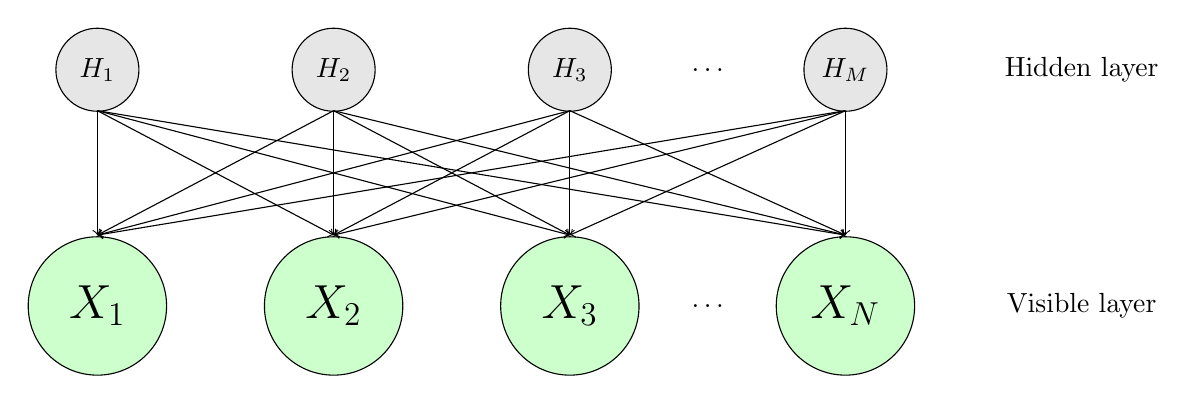
\begin{tikzpicture}
	\draw[black,fill=gray,fill opacity=0.2] (-4.5,0) circle (15pt) node[text=black, fill opacity=1] {$H_1$};
	\draw[black,fill=gray,fill opacity=0.2] (-1.5,0) circle (15pt) node[text=black, fill opacity=1] {$H_2$};
	\draw[black,fill=gray,fill opacity=0.2] (1.5,0) circle (15pt) node[text=black, fill opacity=1] {$H_3$};
	\node[draw, white, text=black] at (3.25,0) {$\dots$};
	\node[draw, white, text=black] at (8,0) {Hidden layer};
	\node[draw, white, text=black] at (8.0,-3) {Visible layer};
	\draw[black,fill=gray,fill opacity=0.2] (5,0) circle (15pt) node[text=black, fill opacity=1] {$H_\text{M}$};
	\draw[black,fill=green,fill opacity=0.2] (-4.5,-3) circle (25pt) node[text=black, fill opacity=1, align= center] {\LARGE $X_1$};
	\draw[black,fill=green,fill opacity=0.2] (-1.5,-3) circle (25pt) node[text=black, fill opacity=1] {\LARGE$X_2$};
	\draw[black,fill=green,fill opacity=0.2] (1.5,-3) circle (25pt) node[text=black, fill opacity=1] {\LARGE$X_3$};
	\node[draw, white, text=black] at (3.25,-3) {$\dots$};
	\draw[black,fill=green,fill opacity=0.2] (5,-3) circle (25pt) node[text=black, fill opacity=1] {\LARGE$X_\text{N}$};
	\draw[black,->] (-4.5,-0.52) to (-1.5,-2.1);
	\draw[black,->] (-4.5,-0.52) to (-4.5,-2.1);
	\draw[black,->] (-4.5,-0.52) to (1.5,-2.1);
	\draw[black,->] (-4.5,-0.52) to (5,-2.1);
	\draw[black,->] (-1.5,-0.52) to (-1.5,-2.1);
	\draw[black,->] (-1.5,-0.52) to (-4.5,-2.1);
	\draw[black,->] (-1.5,-0.52) to (1.5,-2.1);
	\draw[black,->] (-1.5,-0.52) to (5,-2.1);
	\draw[black,->] (1.5,-0.52) to (-1.5,-2.1);
	\draw[black,->] (1.5,-0.52) to (-4.5,-2.1);
	\draw[black,->] (1.5,-0.52) to (1.5,-2.1);
	\draw[black,->] (1.5,-0.52) to (5,-2.1);
	\draw[black,->] (5,-0.52) to (-1.5,-2.1);
	\draw[black,->] (5,-0.52) to (-4.5,-2.1);
	\draw[black,->] (5,-0.52) to (1.5,-2.1);
	\draw[black,->] (5,-0.52) to (5,-2.1);
	\end{tikzpicture}
	\caption{Sketch of a Neural Network Quantum State: it shows the architecture of a Restricted Boltzmann Machine applied to our quantum many-body problem. The visible layer ($X_i$, with $i=1,\dots,$N) is a set of N visible neurons which take as input the positions of the particles, whereas the hidden layer ($H_j$, with $j=1,\dots,$M) is a set of M invisible neurons.}
	\label{Fig:draw}
\end{figure}


The joint probability distribution of the RBM is defined as 
\begin{equation*}
F_{RBM}(\textbf{X},\textbf{H}) = \frac{1}{Z} \exp(-E(\textbf{X},\textbf{H})),
\end{equation*}
where \textbf{X} is the visible nodes and \textbf{H} is the hidden nodes. The quantity $Z$ represents the partition function or normalization constant of the system. 

The quantity $E(\textbf{X},\textbf{H})$ is the function that specifies the relation between the visible and hidden nodes. It is called the energy of the node configuration. This is different from the energy of the quantum mechanical system. The choice of $E(\textbf{X},\textbf{H})$ defines the kind RBM we have. In the bosonic case, the visible nodes need to take continuous values to properly represent the particle positions. We then look at the Gaussian-Binary RBM. In other cases it might be more desirable to have binary outputs (as Carleo and Troyer used for the Ising Model in \cite{carleoSolvingQuantumManybody2017}). For those cases the Binary-Binary RBM can be used. The Gaussian-Binary RBM is given as 
\begin{equation*}
E(\textbf{X},\textbf{H}) = \sum_i^{\text{N}}\frac{(X_i-a_i)^2}{2\sigma} - \sum_j^{\text{M}}b_jH_j + \sum_{ij}^{\text{N,M}}\frac{X_iw_{ij}H_j}{\sigma^2},
\label{eq_rbm}
\end{equation*}
where \textbf{a} is the visible bias, \textbf{b} is the hidden bias and $\textbf{w}_{ij}$ is the weight of the connection between visible node $i$ and hidden node $j$. We have N visible nodes and M hidden nodes. To represent the particle positions, N has to be the number of particles $\times$ the number of dimensions.  The general recipe is to take fewer hidden nodes than the visible ones.

To represent the wave-function, we use the so-called "marginal PDF" found by summing over all the hidden nodes:
\begin{equation*}
\Psi(\textbf{X}) = \sum_HF_{RBM}(\textbf{X},\textbf{H}) = \frac{1}{Z}\sum_H\exp(-E(\textbf{X},\textbf{H})).
\end{equation*}
Setting in the Gaussian-Binary RBM gives the final result
\begin{equation*}
\Psi(\mathbf{X}) = \frac{1}{Z} \exp\bigg[-\sum_i^{\text{N}} \frac{(X_i-a_i)^2}{2\sigma^2}\bigg]\prod_j^{\text{M}} \left(  1 + \exp\bigg[b_j +\sum_i^{\text{N}} \frac{X_iw_{ij}}{\sigma^2}\bigg]\right).
\label{eq_psi}
\end{equation*}
As stated above, the aim of the RBM is to learn a probability. To accomplish this task, the bias $\mathbf{a},\mathbf{b}$ and the weights $\mathbf{w_{ij}}$ need to be modified according to a rule, which in our case is to minimize the energy. We will obtain that some connections between nodes are more weighted than others: in fact, this is the utility of Machine Learning i.e. to understand which connections are more favored than others, this skill could be important in some cases to reduce significantly problems that are impossible to deal with at the beginning.

\subsubsection{Analysis of Hamiltonian}
The local energy is defined as 
\begin{equation*}
E_L = \frac{1}{\Psi(\textbf{X})}\textbf{H}\Psi(\textbf{X}) = \frac{1}{\Psi(\textbf{X})} \left(\sum_{k=1}^{N_p} -\frac{1}{2}\nabla_k^2 + V_{ext}(\mathbf{r}_k)\right)\Psi(\textbf{X})+\sum_{k<i}^{N_p} V_{int}(\mathbf{r}_k,\mathbf{r}_i).
\label{eq_loc_e}
\end{equation*}
Now let us focus on the term $\nabla^2\Psi$. It can be solved analytically. We start by taking the gradient, the derivative is with respect to the visible nodes. We look at the gradient with respect to the coordinates of the $j$'th particle. We begin with using the product rule:
\begin{align*}
\nabla_j\Psi(\textbf{X}) = -\left(\sum_{k=j}^{j+\text{D}}\frac{X_k-a_k}{\sigma^2}\hat{\textbf{X}}_k \right) e^{\sum_i^{\text{N}}\frac{(X_i-a_i)^2}{2\sigma^2}} \prod_l^{\text{M}}\left(1+e^{b_L}e^{\sum_i^{\text{N}}\frac{X_iW_{il}}{\sigma^2}}\right) \\
+ e^{\sum_i^{\text{N}}\frac{(X_i-a_i)^2}{2\sigma^2}} \sum_ {i=j}^{j+\text{D}}\prod_{l\neq j}^{\text{M}} \left(1+e^{b_l}e^{\sum_i^{\text{N}}\frac{X_iW_{il}}{\sigma^2}}\right) e^{b_j}e^{\sum_i^{\text{N}}\frac{X_iW_{il}}{\sigma^2}}\sum_ {k=j}^{j+\text{D}}\frac{W_{kl}}{\sigma^2}\hat{\textbf{X}}_k,
\end{align*}
where $\hat{\textbf{X}}_k$ is the unit vector in the direction of $\textbf{X}_k$ and D is the number of dimensions. We can collect terms and recognize $\Psi(\textbf{X})$ in the expression above. We have
\begin{equation}
\nabla_j \Psi(\textbf{X}) = \Psi(\textbf{X})\left(  -\sum_{k=j}^{j+\text{D}} \frac{X_k-a_k}{\sigma^2} \hat{\textbf{X}}_k  + \sum_{l}^{\text{M}}\frac{e^{b_l}e^{\sum_{i}^{\text{N}}\frac{X_iW_{il}}{\sigma^2}}}{1+e^{b_l}e^{\sum_{i}^{\text{N}}\frac{X_iW_{il}}{\sigma^2}}}  \sum_{k=j}^{j+\text{D}} \frac{W_{kl}}{\sigma^2} \hat{\textbf{X}}_k    \right).
\label{eq_gradient}
\end{equation}
When finding the laplacian it will be convenient to treat the gradient as one expression. Using the product rule we then get
\begin{align*}	
\nabla^2_j \Psi(\textbf{X}) = \frac{(\nabla_j \Psi(\textbf{X}) )^2}{\Psi(\textbf{X})} + \Psi(\textbf{X})\left[ \sum_{k=j}^{j+\text{D}}-\frac{1}{\sigma^2} + \sum_{l=1}^{\text{M}} \frac{e^{b_l}e^{\sum_{i}^{\text{N}}\frac{X_iW_{il}}{\sigma^2}}\sum_{k=j}^{j+\text{D}} \frac{W_{kl}^2}{\sigma^4}  \Big(1+e^{b_l}e^{\sum_{i}^{\text{N}}\frac{X_iW_{il}}{\sigma^2}}\Big)}{\Big(1+e^{b_l}e^{\sum_{i}^{\text{N}}\frac{X_iW_{il}}{\sigma^2}}\Big)^2} \right.  \\ \left. - \frac{ e^{b_l}e^{\sum_{i}^{\text{N}}\frac{X_iW_{il}}{\sigma^2}}\sum_{k=j}^{j+\text{D}} \frac{W_{kl}}{\sigma^2} \hat{\textbf{X}}_k e^{b_l}e^{\sum_{i}^{\text{N}}\frac{X_iW_{il}}{\sigma^2}} }{\Big(1+e^{b_l}e^{\sum_{i}^{\text{N}}\frac{X_iW_{il}}{\sigma^2}}\Big)^2}   \sum_{k=j}^{j+\text{D}} \frac{W_{kl}}{\sigma^2} \hat{\textbf{X}}_k     \right]  \\
= \frac{(\nabla_j \Psi(\textbf{X}) )^2}{\Psi(\textbf{X})} + \Psi(\textbf{X})\left[-\frac{\text{D}}{\sigma^2} + \sum_{l=1}^{\text{M}}  \frac{e^{b_l}e^{\sum_{i}^{\text{N}}\frac{X_iW_{il}}{\sigma^2}}  \Big(1+e^{b_l}e^{\sum_{i}^{\text{N}}\frac{X_iW_{il}}{\sigma^2}}\Big) - e^{b_l}e^{\sum_{i}^{\text{N}}\frac{X_iW_{il}}{\sigma^2}}}{\Big(1+e^{b_l}e^{\sum_{i}^{\text{N}}\frac{X_iW_{il}}{\sigma^2}}\Big)^2}  \sum_{k=j}^{j+\text{D}} \frac{W^2_{kl}}{\sigma^4}      \right]\\
= \frac{(\nabla_j \Psi(\textbf{X}) )^2}{\Psi(\textbf{X})} + \Psi(\textbf{X})\left[ -\frac{\text{D}}{\sigma^2} + \sum_{l=1}^{\text{M}}   \frac{e^{b_l}e^{\sum_{i}^{\text{N}}}\frac{X_iW_{il}}{\sigma^2}  }{\Big(1+e^{b_l}e^{\sum_{i}^{\text{N}}\frac{X_iW_{il}}{\sigma^2}}\Big)^2}  \sum_{k=j}^{j+\text{D}} \frac{W^2_{kl}}{\sigma^4}      \right]
\end{align*}
Finally we wish to look at the laplacian normalized by the wave-function. The result is 
\begin{equation*}
\frac{\nabla_j^2\Psi(\textbf{X})}{\Psi(\textbf{X})}= \left(\frac{\nabla_j \Psi(\textbf{X}) }{\Psi(\textbf{X})}\right)^2 - \frac{\text{D}}{\sigma^2}  + \sum_{l=1}^{\text{M}}   \frac{e^{b_l}e^{\sum_{i}^{\text{N}}}\frac{X_iW_{il}}{\sigma^2}  }{\Big(1+e^{b_l}e^{\sum_{i}^{\text{N}}\frac{X_iW_{il}}{\sigma^2}}\Big)^2}  \sum_{k=j}^{j+\text{D}} \frac{W^2_{kl}}{\sigma^4}     
\label{eq_laplace}
\end{equation*}


\paragraph{Quantum force}
The gradient is already calculated in Eq. (\ref{eq_gradient}). Dividing by $\Psi(\textbf{X})$ we get the quantum force 
\begin{equation*}
\textbf{F}_j = \frac{2\nabla\Psi}{\Psi}=  2\left(  -\sum_{k=j}^{j+\text{D}} \frac{X_k-a_k}{\sigma^2} \hat{\textbf{X}}_k  + \sum_{l}^{\text{M}}\frac{e^{b_l}e^{\sum_{i}^{\text{N}}\frac{X_iW_{il}}{\sigma^2}}}{1+e^{b_l}e^{\sum_{i}^{\text{N}}\frac{X_iW_{il}}{\sigma^2}}}  \sum_{k=j}^{j+\text{D}} \frac{W_{kl}}{\sigma^2} \hat{\textbf{X}}_k    \right).
\label{eq_quantumforce}
\end{equation*}

